\chapter{%
序論}

% 章アブストラクト
本章では,本研究の背景と目的,そして構成について述べる.


\section{研究背景}
 配管は気体、液体、粉粒対などの流体を輸送や配線の保護などを目的とする管のことである。
例を挙げると、電気配線やケーブルを保護する電気配管や生活に必要な水を家庭、学校などに輸送する水道管などに使用されている。
この配管は運用と保護を確保するために、耐久性と安全性を常に保ち続ける必要がある。 \\
BIM とは、Building Information Modeling の略称で、建築物や土木構造物などの情報をコンピュータ上に現実と同じ建物の立体モデルを
形成し、設計から維持管理までのプロセスをデジタル化する新しいワークフローの一環である。このBIMモデリングはこれまでの3Dモデリングとは
大きく異なる。3次元モデルは2次元上で図面を作ってから3次元の形状を組み立てシミュレーションするという流れが主流であった。
そのため、3Dモデルに修正点があった場合に、2Dの図面を全て修正してから構築する必要があり効率的ではなかった。
しかし、このBIMモデルは一つのデータを修正すると全てのデータが連動し、関係する図面の該当箇所が自動修正されるようになるため、従来の
3次元モデルよりも高校率で作業を行うことができる。\\
 本研究においては建築物の中でも配管に焦点をあて、配管のアイソメ図を作成することが最終目標である。アイソメ図を取得するためにはこれまでに
Light Detection and Ranging(LIDAR)センサーと呼ばれるレーザー光を使用して離れた場所にある物体の形状や距離を測定できるセンサーを使用していた。
このセンサーは精度が非常に良いというメリットはあるが、他のセンサーと比較すると高価であるというデメリットを抱えている。そのため、一般的に使用するためには
安価なセンサーでデータ収集ができることが望まれる。また、従来の方法ではセンサーから取得されたデータを手作業で配管を選択することで
アイソメ図を作成していた。手作業による手法は効率が悪いことから、自動で配管を認識できるシステムがが求められる。
このような背景から本研究ではLIDARセンサーの代わりにRGB-Dカメラを用いた深層学習によるアイソメ図の作成を目指す。RGB-DカメラはDepth画像を使用できることから
LIDARセンサー同様に距離情報を取得でき、配管の距離を算出することが可能である。また、LIDARセンサーと比較すると約40倍ほど安価であるため、
たくさんの人が利用しやすいメリットがある。また、深層学習を取り入れることで自動で配管の認識を行い高効率化を目指す。


\section{既存研究}
 アイソメ図を作成するにあたって曲管とT字管の6D姿勢を認識する必要がある。
6D姿勢は座標X、Y、Zに加えYaw、Pitch、Rollの回転情報を加えたものである。その6D姿勢推定を行うネットワークであるGeneralizable 
Model-Free 6-DoF Object Pose Estimation from RGB Images(Gen6D)を紹介する。姿勢推定に必要な主なデータセットは
3次元データやカラー画像、深度データなどが代表的である。しかし、3次元データを生成するためにはオブジェクトの3Dモデルを作る必要があるため、
実用化するのは困難である。Gen6Dネットワークはデータセットを3Dデータを必要とせずカラー画像のみで物体の姿勢推定を行うことができる。
Gen6Dのネットワーク構成について図3に示す。まず、Detectorと呼ばれる工程では参照画像の情報をもとに認識したいオブジェクトの領域を検出する。
これはCNNと呼ばれる畳み込みニューラルネットワークを用いて画像の特徴を抽出し、得られた特徴をもとに領域を予測する。
次の工程である、SelectorではDetectorで得られた領域の画像と最も近い視点を持つ参照画像を複数枚ある中から1つ抽出する。
これは選択された参照画像の視点をテスト画像の視点とほぼ同様とみなし、誤差は生じますがオブジェクトのポーズの初期姿勢を形成する.
最後の工程では先程得られた姿勢の改良を試みる。まず、参照画像から近い視点の画像をさらに6枚選択し、全参照画像間の平均と分散を算出し、
初期に求められた姿勢の情報を改善して最終的な結果を予測する。この研究のメリットとしてRGB画像のみを用意することで物体の姿勢を推定できるため、
データセットの作成は非常に容易である。しかし、このGen6Dをしようするにあたって問題点が2つある。まず、一つ目にRGB画像は距離情報を持たないため、
スケール情報を示さなければならないアイソメ図を作成することが不可能である。そのため、Depth画像を用いることでカラー画像に加え、震度情報が追加されるため
物体間のスケールを算出することが可能である。2つ目は複数の物体を姿勢推定することができない点である。一般的に配管が設置されている現場では、
単体ではなく複数の配管が張り巡らされていることがほとんどであるため、画像内の全ての配管を網羅し認識することが要求される。
これを解決するためにはGen6DのDetectorを複数物体検出可能なネットワークに変更する必要がある。\\
 そのDetectorを複数物体検知可能にするにあたって、2次元上で複数の物体検出を可能にするYOLOV3を紹介する。このモデルはほぼ同時期に発表された
 Fast R-CNNと同様に、物体検出に大きな影響を与えた。これ以降、End-to-Endモデルとリアルタイム検出が物体検出の中で主流となった。
YOLOの特徴は従来までは境界設定と物体検出を2段階に行っていた作業を一度に行うことで推定速度の高速化を行うことができた。図1.2に
YOLOの物体検出までの流れを示す。\\
まず、入力画像をS*Sのグリッドセルに分割する。物体の中心がグリッドセルに存在していた場合に、そのセルが物体を検出するように学習する。
次に、バウンディングボックスの推定では各グリッドセルにB個のバウンディングボックスを持ち、それらのボックスの信頼スコアを予測する。
信頼スコアとは背景ではなく物体が含まれている確率のことである。次に、各グリッドセルは複数のクラスに対する条件付き確率を予測する
算出された条件付きクラス確率と一つ前の個々のバウンディングボックスの信頼スコアを掛け合わせることで、バウンディングボックス毎の
クラスに対する信頼スコアを得ることができる。このスコアを使用しどのバウンディングボックスが正解の物体を推定しているのかを判断する。

\begin{figure}[htbt]
	\centering
	 \includegraphics[height=55mm]{gen6d-network.eps}
	 \caption{Gen6Dネットワーク構造}
	 \label{fig:f2}
\end{figure}

\begin{figure}[htbt]
	\centering
	 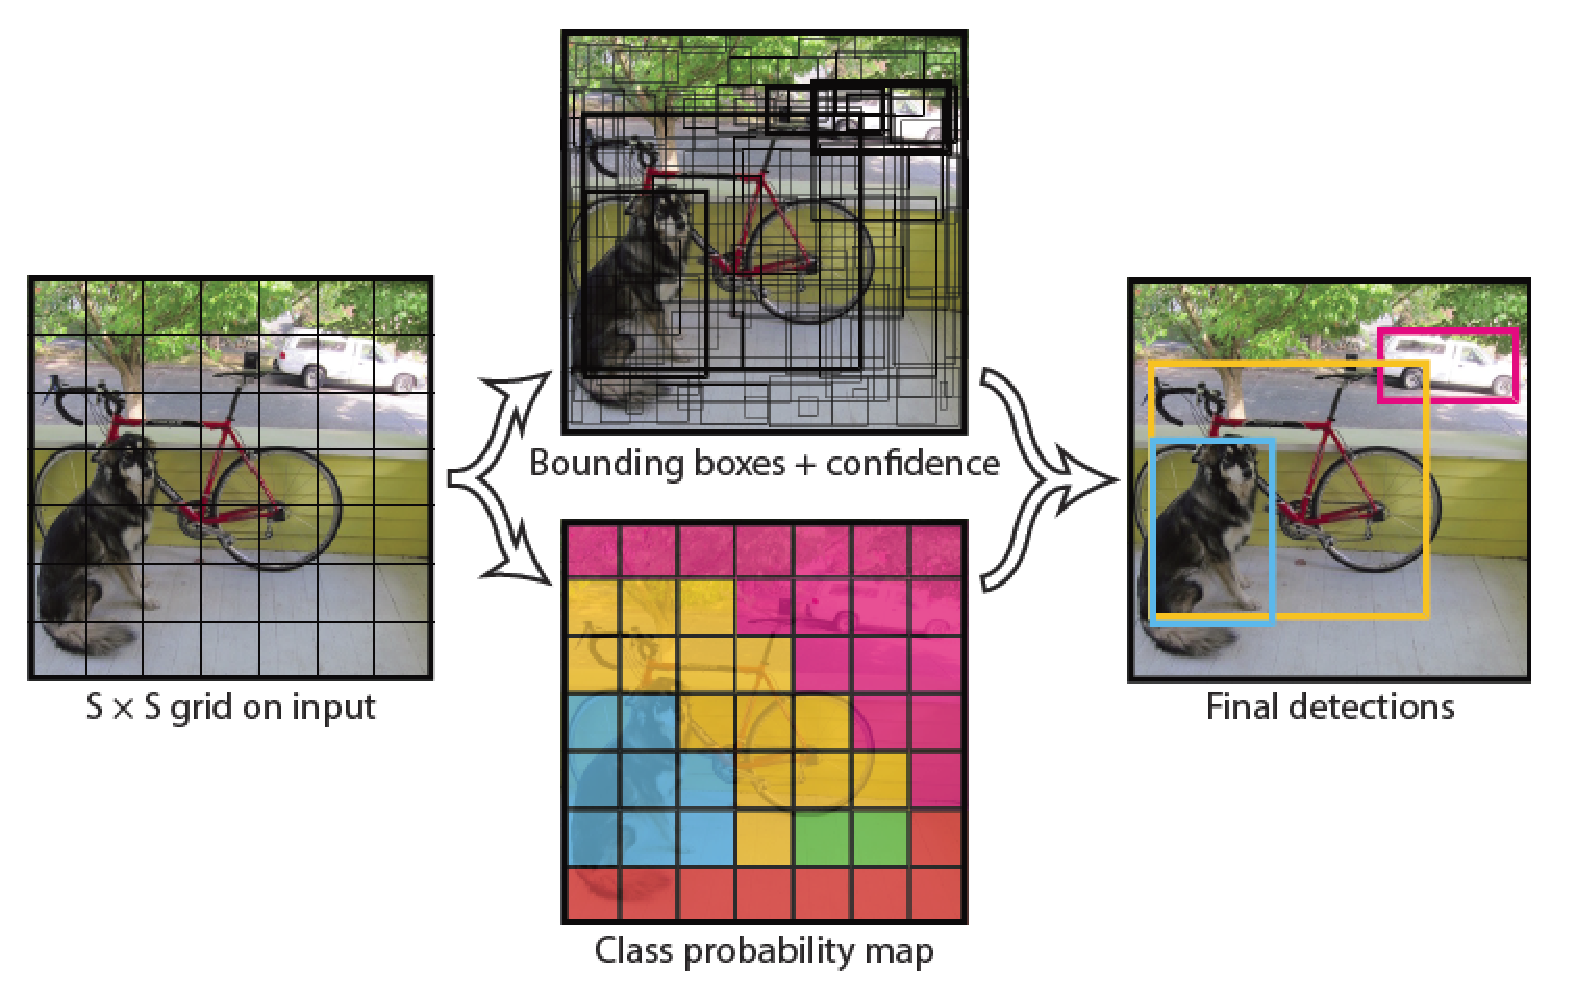
\includegraphics[height=75mm]{yolo.eps}
	 \caption{YOLOモデルの検出の流れ}
	 \label{fig:f2}
\end{figure}

\section{研究目的}
 本研究ではRGBDデータを使用した深層学習による配管6D姿勢推定を行い、RGBDカメラを用いることによる安価な機器での姿勢推定の実現を試みる.
また,既存のRGB画像のネットワークにDepth画像を組み込んだモデルを提案し、認識精度向上と推定速度の高速化を目標とする。
本研究の貢献は以下のようになる。まず一つ目は深層学習によるRGB画像とDepth画像より物体検出ネットワークの提案である。
特に、RGB画像とDepth画像からそれぞれ抽出された特徴を結合するRxDLayerを導入し、ネットワーク性能の向上させた。
他のネットワークと精度を比較することで提案ネットワークの有効性を検証した。\\
2つ目は既存の6D姿勢推定ネットワークに複数物体検出を可能にさせたことである。配管は単体ではなく複数の管が張り巡らされているため、複数の
認識を可能にする必要がある。提案ネットワークでは画像内部にある配管全てを網羅し、それぞれの物体の中心ピクセル座標とスケールを推定することができる。
3つ目は本研究の最終目的であるアイソメ図を作成するにあたっての必要不可欠な配管距離測定である。アイソメ図は配管の向きだけでなく、距離情報を図面に
示す必要がある。そのため、Depth画像を用いることでネットワークによって認識された情報をもとに、配管の距離情報を算出することを可能にした。

\section{本手引の構成}
 本論文の構成は以下のようになる。第一章では研究背景、既存研究、研究目的について述べる。研究背景では、
Building Information Modeling(BIM)についてやRGB-Dカメラを使用するメリットについて述べる。
既存研究では、配管6D姿勢推定と物体検出のそれぞれのネットワークを紹介する。
それぞれのネットワークのメリットやデメリットをもとにアイソメ図に必要となるネットワーク設計を述べる。
研究目的では、本研究の目的及び貢献について述べる。
 第2章では,論文の論理構成をどのようにすべきかを述べる.
第3章では,論文の体裁について述べる.
第4章では,論文作成および研究一般におけるその他の重要な注意点について述べる.
第5章は結言である.
